\documentclass[a4paper,11pt]{article}
\usepackage[utf8]{inputenc}
\usepackage[T1]{fontenc}
\usepackage[english]{babel}
\usepackage{times}
\usepackage{graphicx}
\textwidth=6in
\textheight=9.0in
\headheight=0in
\headsep=0in
\oddsidemargin=0in
\evensidemargin=0in
\title{Analysis of the SMR-4 VCF/VCA board\\Second design revision}
\author{Olivier Gillet \\ \tt olivier@mutable-instruments.net}
\date{}
\begin{document}

\maketitle

The SMR-4 mkII board is the second revision of the ``default" analog signal processing board for the  Shruthi-1. It includes a 4-pole VCF (presented in section \ref{sec:vcf}) with VC-resonance and a linear VCA (presented in section \ref{sec:vca}); and only makes use of inexpensive and easily available chips.

\section{Generalities}

\subsection{Power}

The board is powered from a non-regulated single supply rail in the 7.5V-15V range. A negative rail is obtained from this by means of a LT1054 DC-DC converter; charged into a $100\mu F$ capacitor -- or $110\mu F$ equivalent when a $10\mu F$ tantalum cap is added in parallel -- and set to a switching frequency of 50kHz. The input positive rail and the negative rail from the LT1054 are regulated by 7805/7905 linear regulators and generously filtered.

The main advantage of working with +/- 5V rails is that no extra regulator is required for powering the digital section. Furthermore, the device can be powered by a 9V battery, or even a pack of five 1.5V batteries. The main drawback is the smaller headroom for all the op-amps -- the LT074 clips at around $\pm 3.7V$.

\subsection{Input signals}

All input signals, be it the raw oscillators signal or the control voltages, are $0$ / $5V$ PWM signals with a carrier frequency of $\frac{20MHz}{510} = 39215 Hz$.

This implies that the control signals have to be smoothed. You should not feel bad about it: the MCU generates the control signals at a ``slow" rate of $980 Hz$ anyway, so a simple 1-pole low-pass with a cutoff frequency of $723 Hz$ kills the PWM carrier by $35dB$ while still tracking fast enough the fastest transitions the MCU can create.

The oscillators signal also has this $39kHz$ carrier. It is attenuated by the main 4-pole LPF itself, and to some extent by the excessively large ``stability" caps in the mixer and VCA I to V converter. In the worst case (cutoff set to its maximum value), the carrier is thus attenuated by $30dB$. In most cases, however, the cutoff frequency is set to a lower value, and the carrier is attenuated more strongly. Anti-aliasing filters at the input of your soundcard, speakers with a limited bandwidth, or your ears will be doing the rest of the filtering. This residual of the PWM carrier might however a bit of parasitic hiss if the output signal is fed into a ``vintage" sampler of FX processor with no anti-aliasing filter (the frequency of the hiss being dependent on the difference between the sampling rate and $39kHz$).

All those considerations are not relevant when the SMR-4 is used with another signals source than the Shruthi-1 control board -- besides justifying the design choices.

\section{VCF}
\label{sec:vcf}

The VCF section consists of a ``CV-scaling" section inverting and scaling the input CV to a range of values suitable for the exponential current source that follows. The exponential current source generates biasing currents for 4 OTA-integrator cells, each of those implementing a 1-pole low-pass filter.

\subsection{OTA-integrator low-pass cell}
\label{sec:otac}

Each ``OTA-integrator" cell of the VCF section follows the template shown in figure \ref{fig:otac}. $R_{37}$ and $R_{39}$, or their counterparts in the other cells, have an identical big value noted $R_b$ ; $R_{35}$ a small value noted $R_s$. $C$ will denote the value of $C_{33}$.

\begin{figure}
\centering
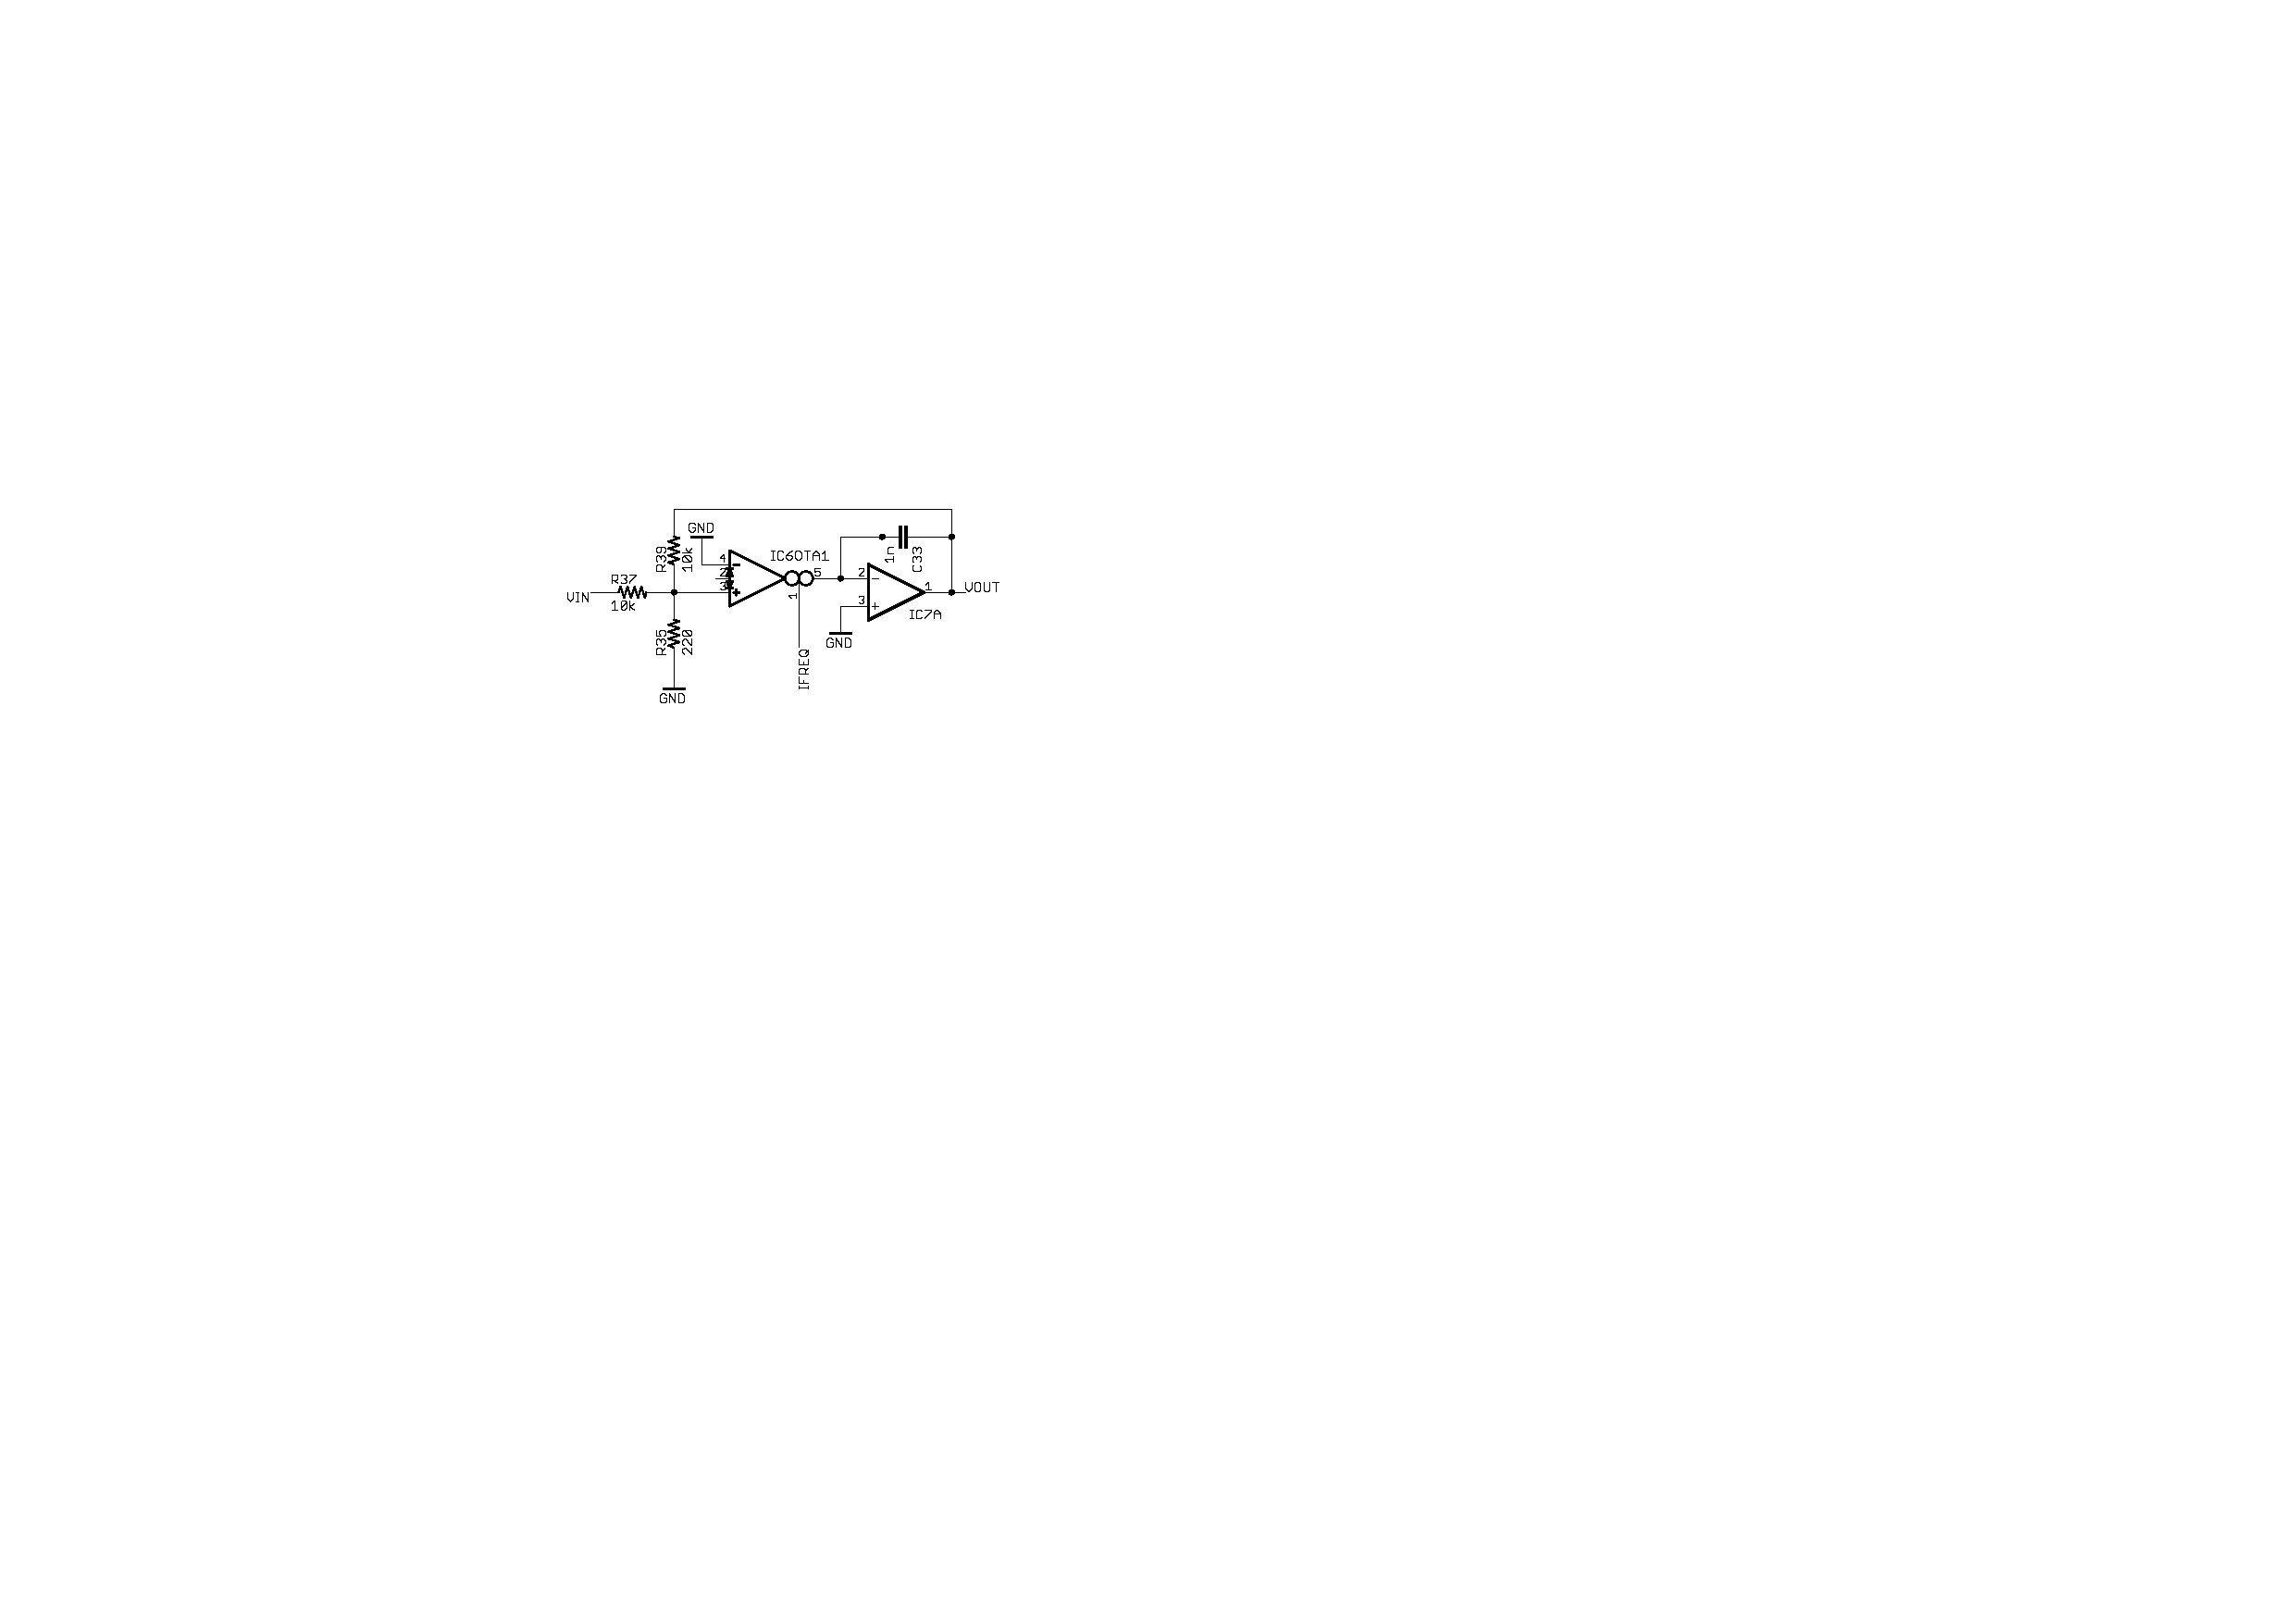
\includegraphics[width=0.8\textwidth]{smr4mkII_otac_cell.pdf}
\caption{OTA-integrator low-pass cell.}
\label{fig:otac}
\end{figure}

Let us start by the OTA. Kirchoff in $V_+$ yields:

\begin{eqnarray}
\frac{1}{R_b}(V_{in}(p) - V_+(p)) + \frac{1}{R_b} (V_{out}(p) - V_+(p)) &=& \frac{1}{R_s} V_+(p) \\
V_+(p) &=& \frac{R_s}{R_b + 2 R_s} (V_{in}(p) + V_{out}(p))
\end{eqnarray}

$V_-$ is simply grounded. The current $I_c(p)$ at the output of the OTA is:

\begin{eqnarray}
I_c(p) &=& g_m (V_+(p) - V_-(p)) \\
 &=& 19.2 I_{freq} \frac{R_s}{R_b + 2 R_s} (V_{in}(p) + V_{out}(p))
\end{eqnarray}

The operational amplifier $IC_{8D}$ is in a simple inverting ``current to voltage" configuration:

\begin{eqnarray}
V_{out}(p) &=& - I_c(p) Z_{feedback}(p) \\
 &=& - \frac{I_c(p)}{Cp} \\
 &=& - 19.2 I_{freq} \frac{R_s}{(R_b + 2 R_s)Cp} (V_{in}(p) + V_{out}(p))
\end{eqnarray}

Solving for $V_{out}(p)$ and dividing by $V_{in}(p)$, we find the transfer function:

\begin{eqnarray}
H(p) &=& \frac{-1}{1 + \frac{(R_b + 2 R_s)}{R_s} Cp \frac{1}{19.2 I_{freq}}}
\end{eqnarray}

The pole is at the frequency $f$ such that:

\begin{eqnarray}
0 &=& 1 + \frac{(R_b + 2 R_s)}{R_s} C 2\pi f \frac{1}{19.2 I_{freq}} \\
f &=& -\frac{19.2 I_{freq}}{2 \pi \frac{(R_b + 2 R_s)}{R_s} C}
\end{eqnarray}

At this stage, we can already pick values for $R_b$, $R_s$, $C$ and design the exponential current source so that its current range translate into a target frequency range using the formula above.

The values that have been chosen for $R_b$, $R_s$ and $C$ follow closely those given in the application schematics of the SSM2040 datasheet (Figure 9 of the datasheet):

\begin{eqnarray*}
R_b &=& 10 k \Omega \\
R_s &=& 220 \Omega \\
C &=& 1 nF
\end{eqnarray*}

$R_s = 200 \Omega$ in the SSM2044 datasheet, but we have privileged here values in the E12 series.

\subsection{Exponential current source}

As explained in the previous section, the cutoff frequency is proportional to the biasing current $I_{freq}$ of the OTAs. Since we want to achieve an exponential frequency control, we need to produce a control current which is an exponential function of the input CV. This is achieved by the exponential current source in figure \ref{fig:expo}.

\begin{figure}
\centering
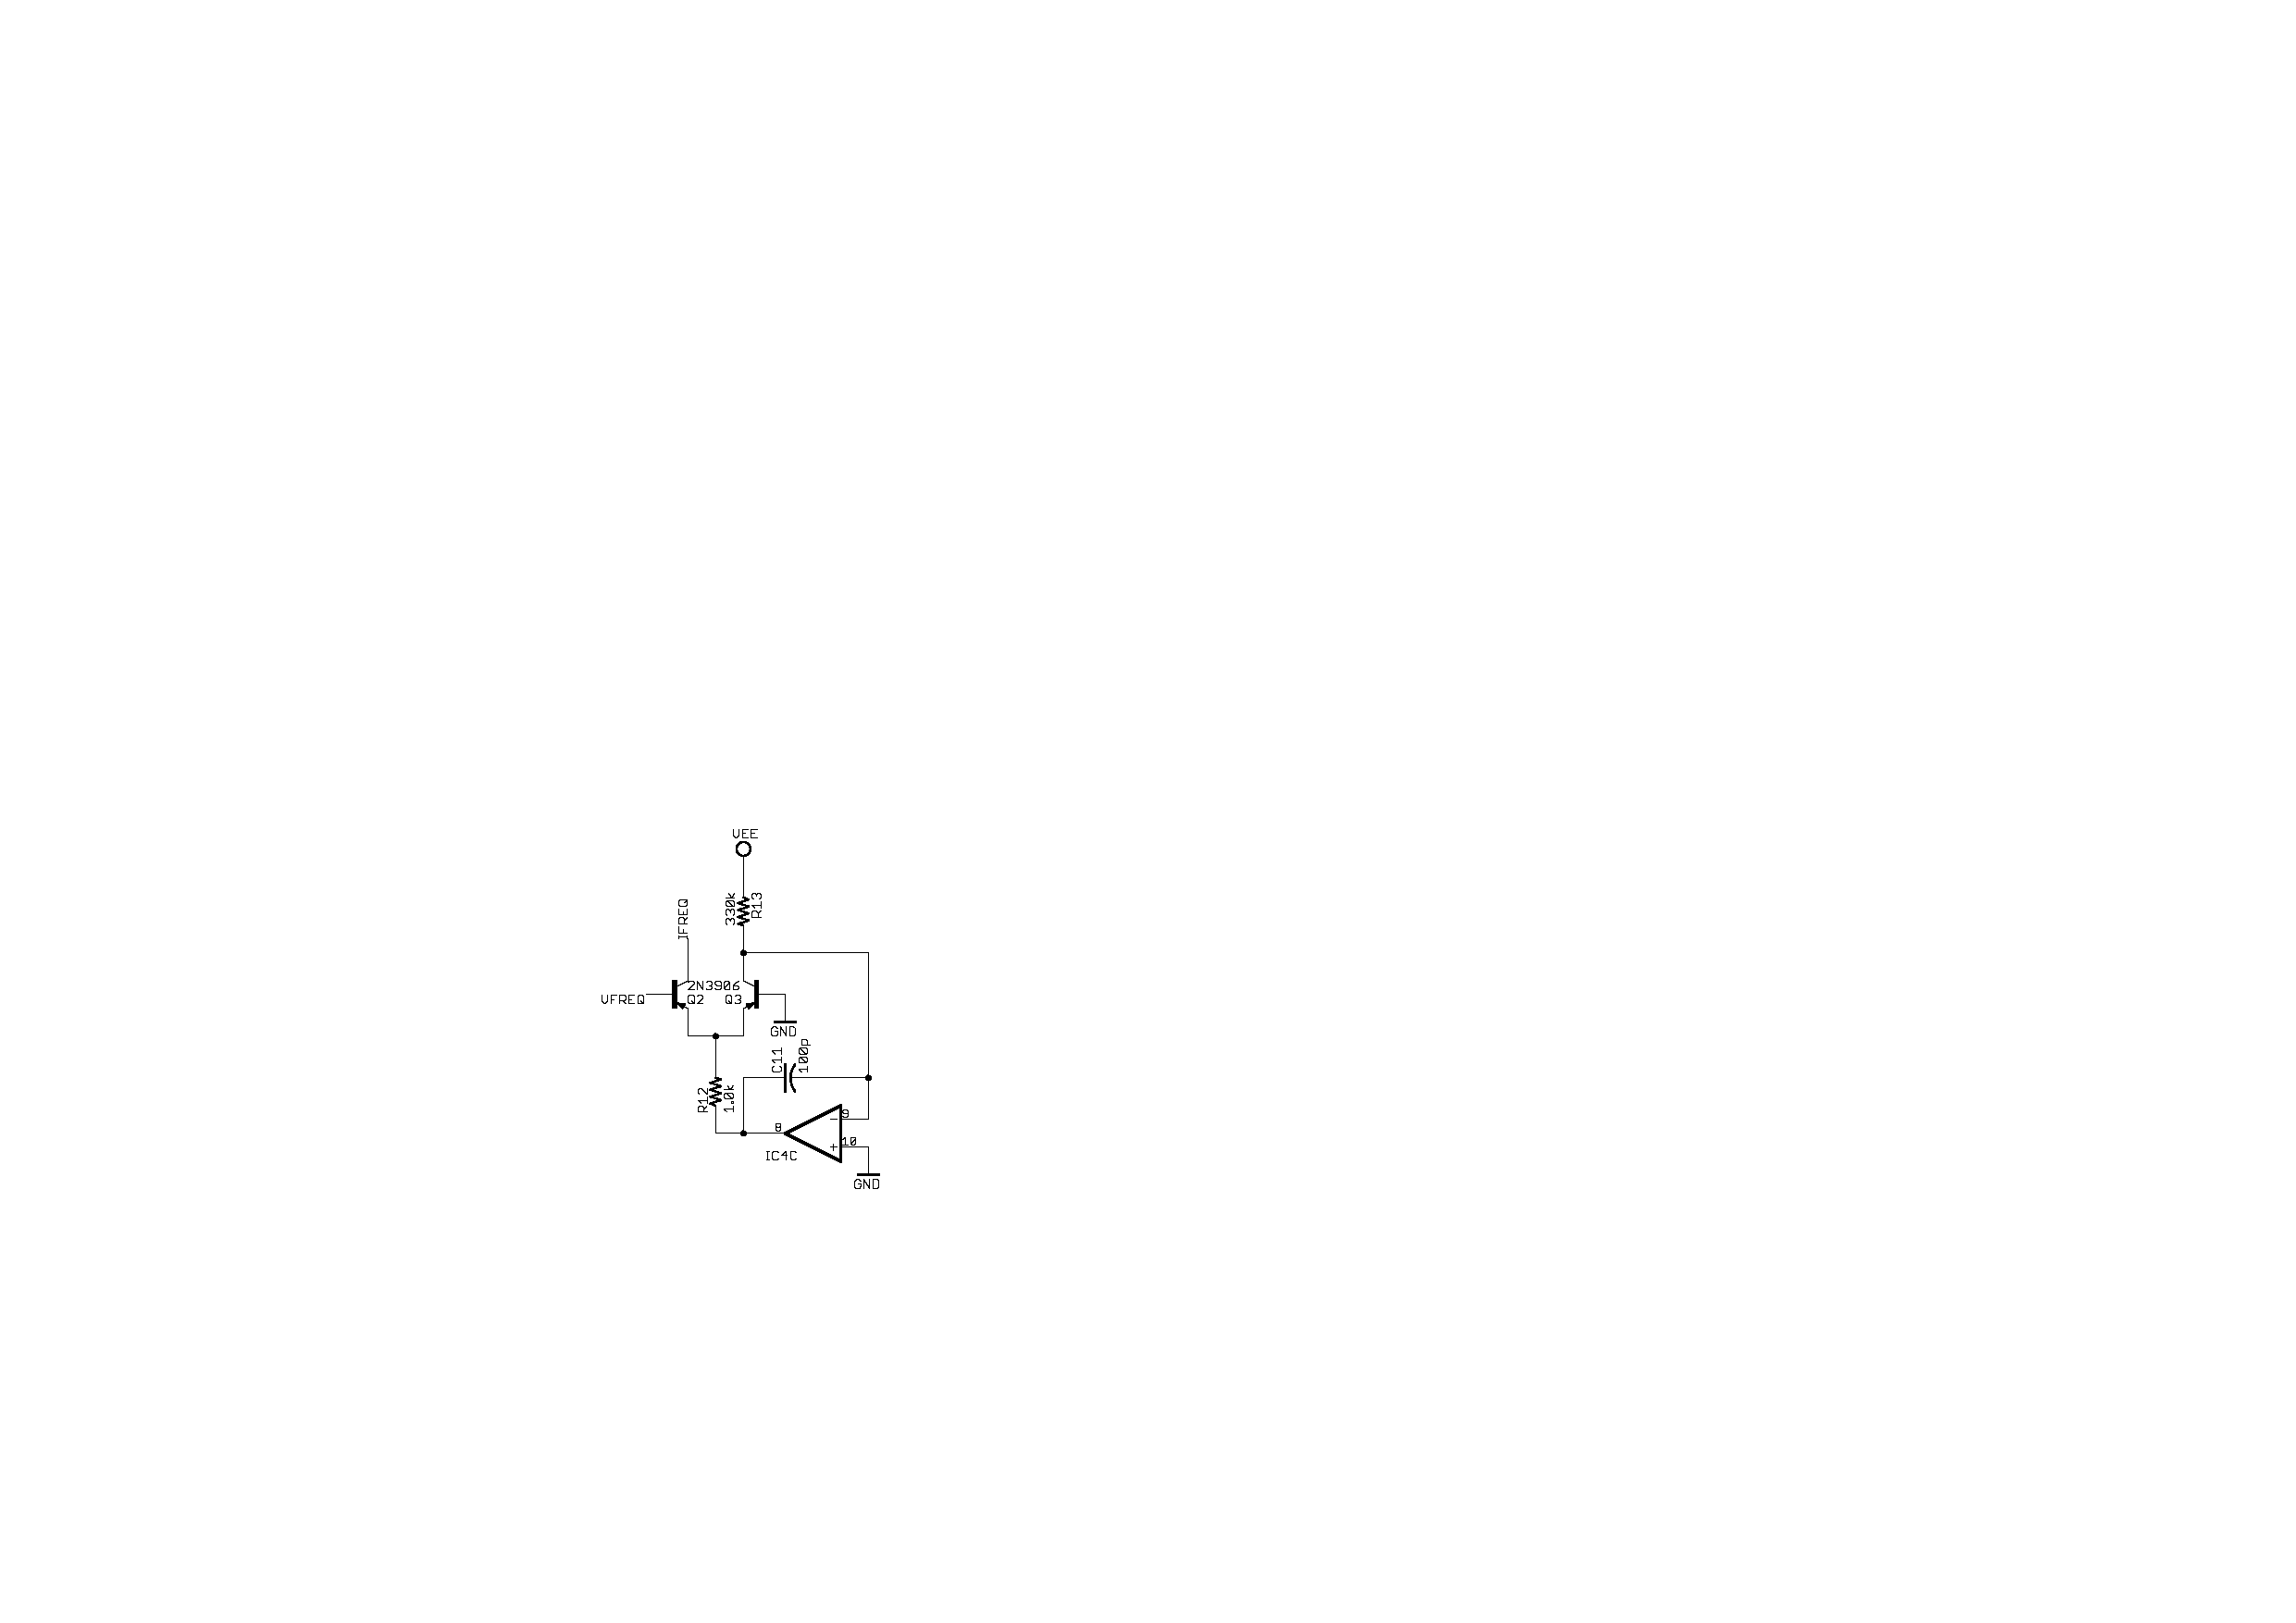
\includegraphics[width=0.5\textwidth]{smr4mkII_expo_current_source.pdf}
\caption{Exponential current source.}
\label{fig:expo}
\end{figure}

Let us start with the core of the circuit -- the PNP transistor pair $Q_2$ and $Q_3$. The Ebers-Moll equations for $Q_2$ and $Q_3$ give the collector currents for both transistors:

\begin{eqnarray}
I_{c2} &=& I_{s2} \left(\exp \left( \frac{V_{eb2}}{V_T} \right) - 1 \right) \\
I_{c3} &=& I_{s3} \left(\exp \left( \frac{V_{eb3}}{V_T} \right) - 1 \right)
\end{eqnarray}

$V_T$ is the thermal voltage, equal to $26 mV$ at room temperature. We will see later that $\exp \left( \frac{V_{eb2}}{V_T} \right)$ is an order of magnitudes bigger than 1, it is thus a sane approximation to ignore the $- 1$ term. Assuming that the two transistors have the same characteristics, $I_{s2} = I_{s3}$. Thus we have, by substituting in the first equation the value of $I_{s2}$ derived from the second one:

\begin{equation}
I_{c2} = I_{c3} \exp \left( \frac{V_{eb2} - V_{eb3}}{V_T} \right)
\end{equation}

Since the base of $Q3$ is grounded, and since the emitter of $Q_2$ and $Q_3$ are at the same potential:

\begin{equation}
V_{eb2} - V_{eb3} = V_{e2} - V_{b2} - V_{e3} + V_{b3} = -V_{b2} = -V_{freq}
\end{equation}

The value of $I_{c3}$ is simply:

\begin{equation}
I_{c3} = \frac{V_{ee} - V_{c3}}{R_{13}} = \frac{V_{ee}}{R_{13}}
\end{equation}

$V_{c3}$ is null because the collector of $Q_3$ is virtually grounded. Indeed, the whole point of the operational amplifier $IC_{4C}$ is to keep the collector of $Q_3$ at a constant potential. $C_{11}$ is only here to stabilize the op-amp. $R_{12}$ works as a current limiter; we can assume that it has no influence in normal operation.

To summarize the previous steps:

\begin{equation}
I_{freq} = -\frac{V_{ee}}{R_{13}} \exp \left(\frac{-V_{freq}}{V_T} \right)
\end{equation}

Observe that the biasing current $I_{freq}$ varies in the inverse direction of $V_{freq}$~-- when $V_{freq}$ increases, $I_{freq}$ decreases. This is not a problem because $V_{freq}$ is generated by an op-amp in an inverting configuration.

One thing not discussed here is temperature compensation. While the main temperature dependent factors (saturation currents) have been neutralized by the ``transistor pair" design (as long as the transistors are of a similar kind and thermically coupled), there remains a temperature dependent term, $V_T$. This term is not compensated. A rough estimate of the variation in frequency is less than $\pm 10\%$ for a change in temperature of $\pm 5^oC$~-- not good for a VCO, but acceptable for a VCF.

\subsection{CV scaling}

The CV scaling stage is fed with a 0/5V PWM signal generated by the microcontroller, and generates a scaled voltage which will translate into an appropriate cutoff frequency range. In addition to the scaling itself, it also actively smoothes the high-frequency PWM control signal into a near-DC voltage. Its schematics are given in figure \ref{fig:cvscale}.

\begin{figure}
\centering
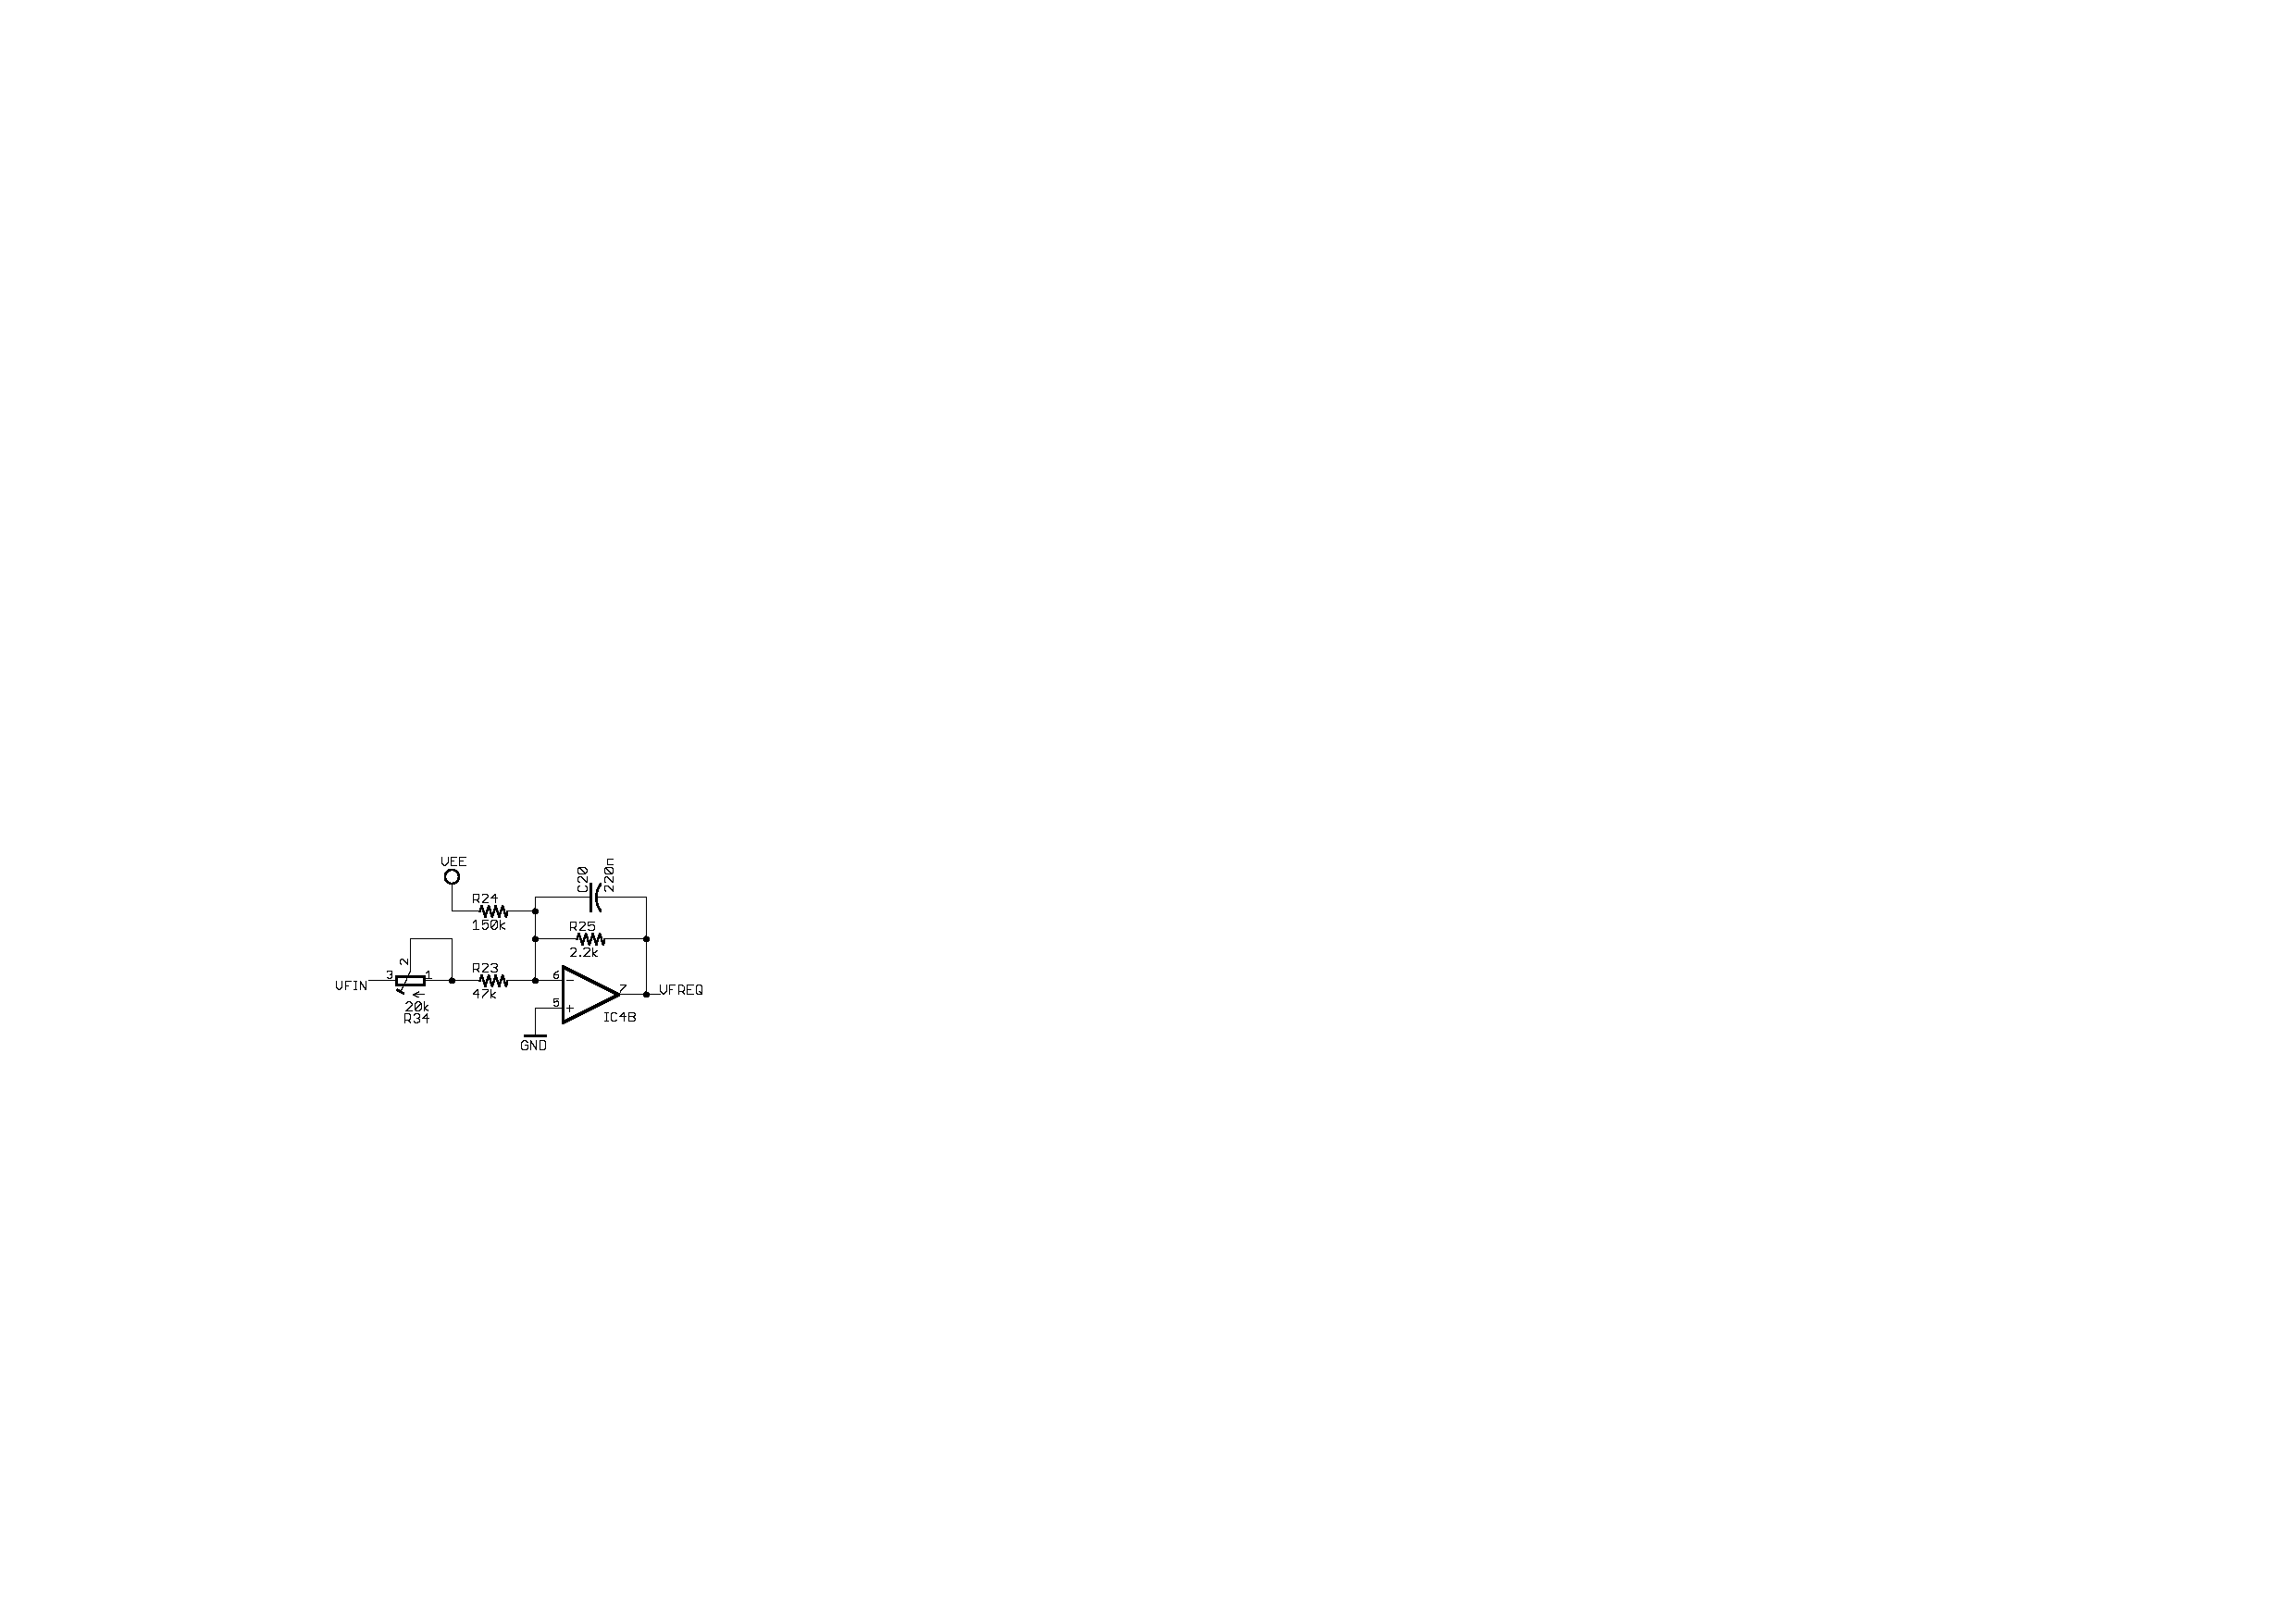
\includegraphics[width=0.8\textwidth]{smr4mkII_scaling.pdf}
\caption{CV-scaling.}
\label{fig:cvscale}
\end{figure}

The voltage at the output of the op-amp is given by:

\begin{equation}
V_{freq}(p) = -\frac{R_{25}}{R_{24}} V_{fin} -\frac{Z_f(p)}{R_{20} + R_{23}} V_{fin}(p)
\end{equation}

Where $Z_f(p)$ is the equivalent impedance of the feedback loop, consisting of $R_{25}$ in parallel with $C_{20}$. Note that in the first term, this impedance is simply $R_{25}$ since the capacitor in parallel with the resistor has no effect on DC currents. In the second term, it is equal to:

\begin{equation}
Z_f(p) = \frac{R_{25}}{1 + R_{25}C_{20}p}
\end{equation}

Thus, the cutoff frequency of the filter smoothing the PWM control signals is $\frac{1}{2 \pi R_{25}C_{20}} = 329 Hz$ with the values given on the schematics. This means that the PWM carrier is attenuated by $6\log_2 \frac{39215}{329} = 40dB$. Given this (moderately) high attenuation factor, it is safe to consider that when the cutoff value is constant, the circuit behaves as if $V_{fin}$ is a pure DC component in the $[0, 5]V$ range instead of a PWM signal.

Note that the use of a supply rail ($V_{ee}$) to generate a negative reference voltage is not a very good practice. This makes the circuit vulnerable to ripples/noise in the negative rail ; and requires accurate voltage regulators. In practice, we have not observed significant noise/ripples on the negative rail ; and small random fluctuations of the cutoff are much less perceptible than noise.

\subsection{An important consideration}

All the computations in the previous steps are done under the assumption that the exponential current source is connected to only one OTA. In the SMR4 mkII filter, the exponential converter is connected to 4 OTAs. Assuming the OTAs have similar characteristics, the biasing current $I_{freq}$ received by each OTA is only one fourth of the value of $I_{c2}$.

This saves 3 transistors but has a drawback: in case one of OTA cells fails, the current received by the other cells will be higher. Under some circumstances (incorrectly trimmed filter and maximum cutoff), this excess of current could damage the remaining cells.

\subsection{Component values}

\subsubsection{Constraints}

How are the different values of the component selected? From the past sections, some characteristics of the ICs used in the circuit, and some common sense, we can gather a set of constraints ($\sim$ denotes an order of magnitude in this section) the component values must satisfy:

\paragraph{Input impedance} The input impedance of the CV scaling circuit $R_{23} + R_{34}$ should not be too low, at least $\sim 10k \Omega$.

\paragraph{OTA small biasing current constraint} The biasing current of the OTA should not exceed $2mA$.

\paragraph{Cutoff frequency constraint} The frequency range of the filter must span the audible spectrum ($20 Hz$ to $20kHz$), and it should be easy to ``tune" it to the fundamental frequency of the oscillators. To this effect, we have decided to eschew the $1 V/octave$ standard (which would have given a very narrow frequency range given that the input signal is in the $[0, 5]V$ range, and to use another approach.

In the Shruthi-1 firmware, the filter tracking code works the following way: the MIDI note value (an integer between 0 and 127) minus 64 is added to the filter cutoff value (which is itself represented as a 7-bit integer). In other words, if the base cutoff setting of the Shruthi-1 is set to $n$, the PWM control signal corresponds to a smoothed DC voltage of:

\begin{equation}
V_{fin} = V_{cc} \frac{n + \mbox{Midi note number} - 64}{128}
\end{equation}

From this, it appears that if we want a 1:1 tracking of the filter frequency to the fundamental frequency of the oscillators, the cutoff frequency should be multiplied by a semitone ($2^\frac{1}{12}$) every time the Midi note number is increased by $1$, that is to say everytime $V_{fin}$ steps by a $\frac{5}{128}$ increment. This yields the rather odd scale of $0.46875V.oct^{-1}$, which is the target $V.oct^{-1}$ scale of the filter.

The filter is thus expected to cover a range of $\frac{128}{12} = 10.66$ octaves~-- the highest cutoff value will be 1625 times the lowest cutoff value. The $14.9 Hz$ -- $22.8kHz$ range has this exact ratio and spans the audible range.

\paragraph{Pragmatic constraints} Resistor values should be preferably in the E12 series ; and the number of distinct component values should be minimized.

\subsubsection{Validation}

We provide in the rest of this section a validation of the selected values.

\paragraph{Input impedance} Greater than $30k\Omega$, all good!

\paragraph{OTA small current constraint} The worst case corresponds to the maximum cutoff value, which can be obtained with an input signal $V_{fin} = 5V$, and $R_{34}$ trimmed to $20k\Omega$. In this case, $V_{freq} = -161mV$ and $I_{c2} = 7.4mA$, yielding $I_{freq} = 1.8mA$ per OTA, below the $2mA$ maximum rating.

\paragraph{Cutoff frequency range} Let us check first that the lowest cutoff frequency attainable with the filter has the expected value. When $V_{fin} = 0V$, $V_{freq} = -73mV$ and $I_{freq} = 0.23\mu A$. The lowest cutoff frequency is thus: $14.5 Hz$.

Let us now check what is the maximum cutoff frequency that can be reached. $V_{fin}$ is now set to $5V$. Depending on how $R_{34}$ is trimmed, we have:

\begin{eqnarray}
0 \Omega \leq &R_{34}& \leq 20 k\Omega \\
91mV \leq &V_{freq}& \leq 161mV \\
0.125 mA \leq &I_{freq}& \leq 1.85 mA \\
8.0kHz \leq &f& \leq 118kHz
\end{eqnarray}

The target frequency range is thus feasible. Note that the exact 1:1 tracking is achieved with $R_{34} = 10.2 kHz$, so the default factory position of the trimmer (middle) is roughly the right one.

\section{VCA}
\label{sec:vca}

\subsection{Linear current source}

\begin{figure}
\centering
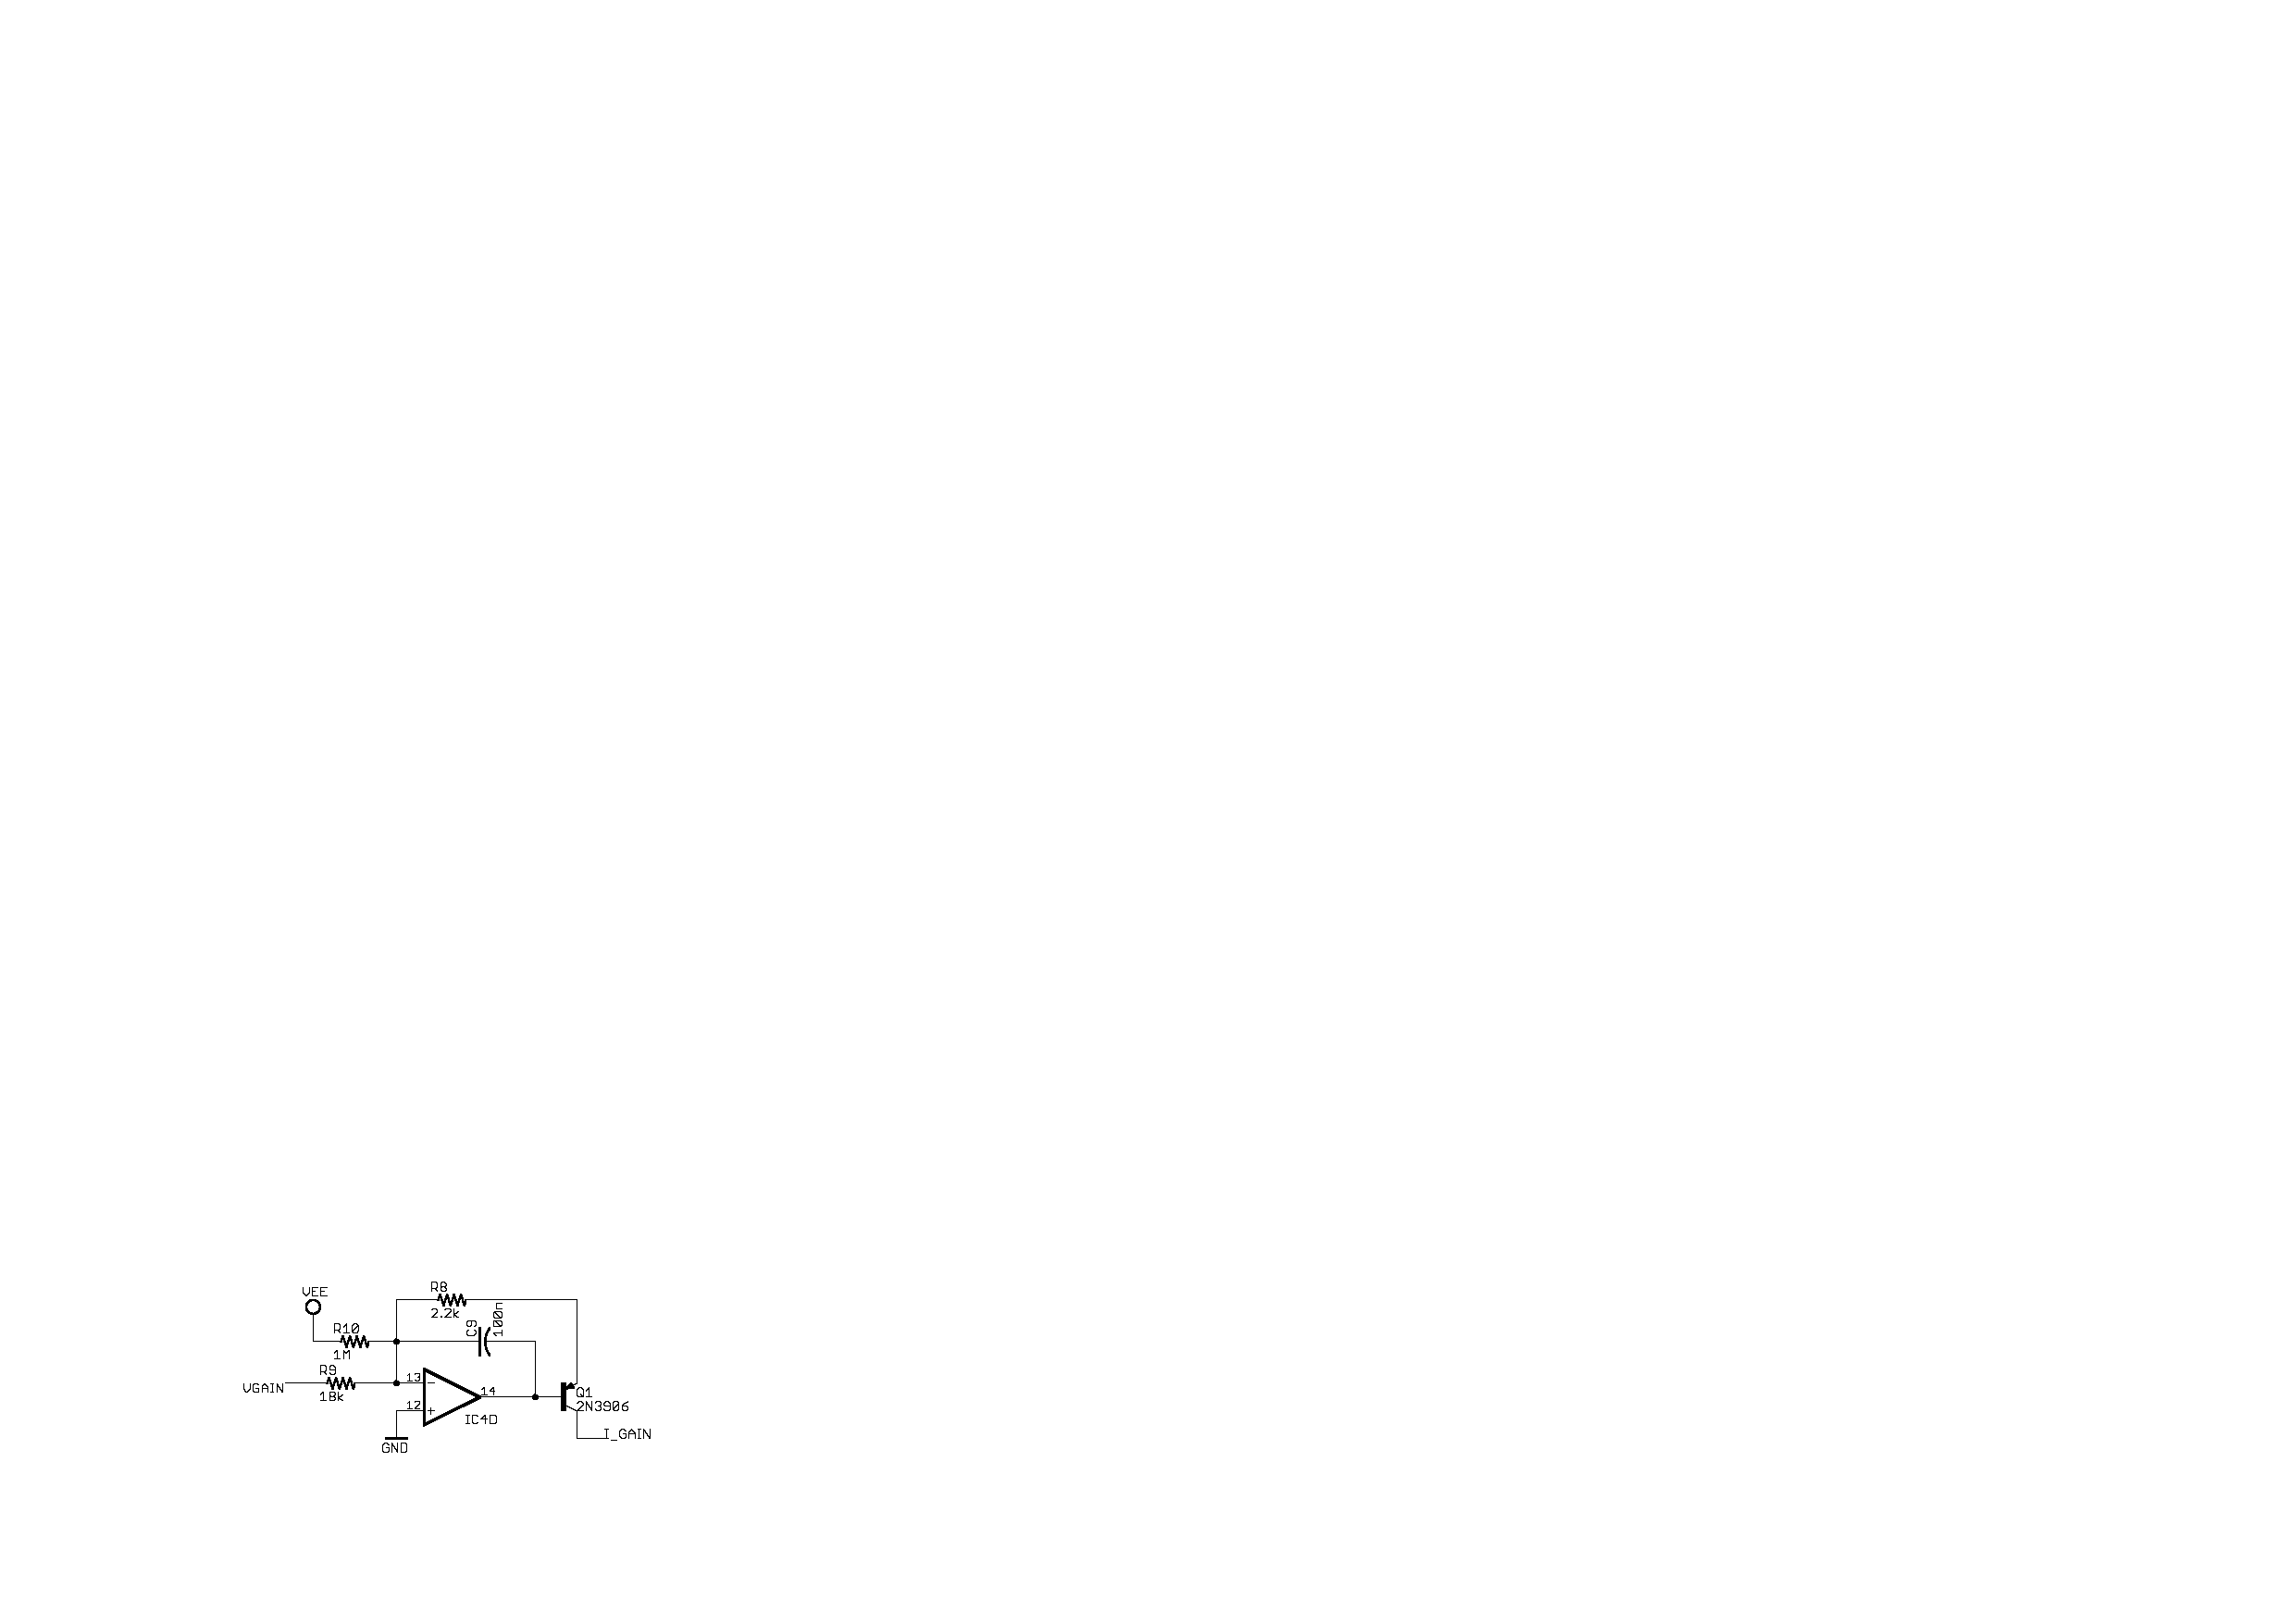
\includegraphics[width=0.7\textwidth]{smr4mkII_linear_current_source.pdf}
\caption{Linear current source.}
\label{fig:linear}
\end{figure}

The linear current source in figure \ref{fig:linear} generates the biasing current for the VCA OTA cell. Let us make a few assumptions:
\begin{itemize}
\item The input signal is DC, and thus, $C9$ has no effect (actually its purpose is to smooth the output).
\item $Q_1$ has an $\alpha$ equal to 1, which implies that $I_{gain} = I_{c1} = I_{e1}$.
\item The op-amp is not operating in saturation mode, which implies that $V_- = V_+ = 0$.
\item The op-amp has infinite input impedance, which implies that $I_- = 0$.
\end{itemize}

Thus, we have:

\begin{equation}
I_{gain} = I_{e1} = I_{R8} = \frac{V_{gain}}{R_9} + \frac{V_{ee}}{R_{10}}
\end{equation}

Intuitively, this circuit works the following way: through feedback, the op-amp ensures that the current flowing through $R_8$ is the same as the input current at the summing node -- it does so by controlling the base voltage of $Q_1$. We have put all the unknown parameters of the Ebers-Moll equation for $Q_1$ giving $I_{c1}$ as a function of $V_{be1}$ (temperature, saturation current) under feedback control!

$I_{gain}$ is thus directly proportional to $V_{gain}$. The additional offset term $\frac{V_{ee}}{R_{10}}$ helps ``silencing" the VCA -- the reason behind this is that the Shruthi-1 control board cannot actually output null voltages -- when a PWM output on the MCU is set to 0 it outputs a few $mV$.

$R_8$ ; in conjunction with the op-amp's clipping ; can play the role of a current limiter on the output current, yielding a kind of reverse-exponential response with a ``knee" when the op-amp starts failing to set its output high or low enough to guarantee that a large enough current flows through the transistor. The value chosen here is low enough to not cause current limiting.

\subsection{Current controlled amplifier}

\begin{figure}
\centering
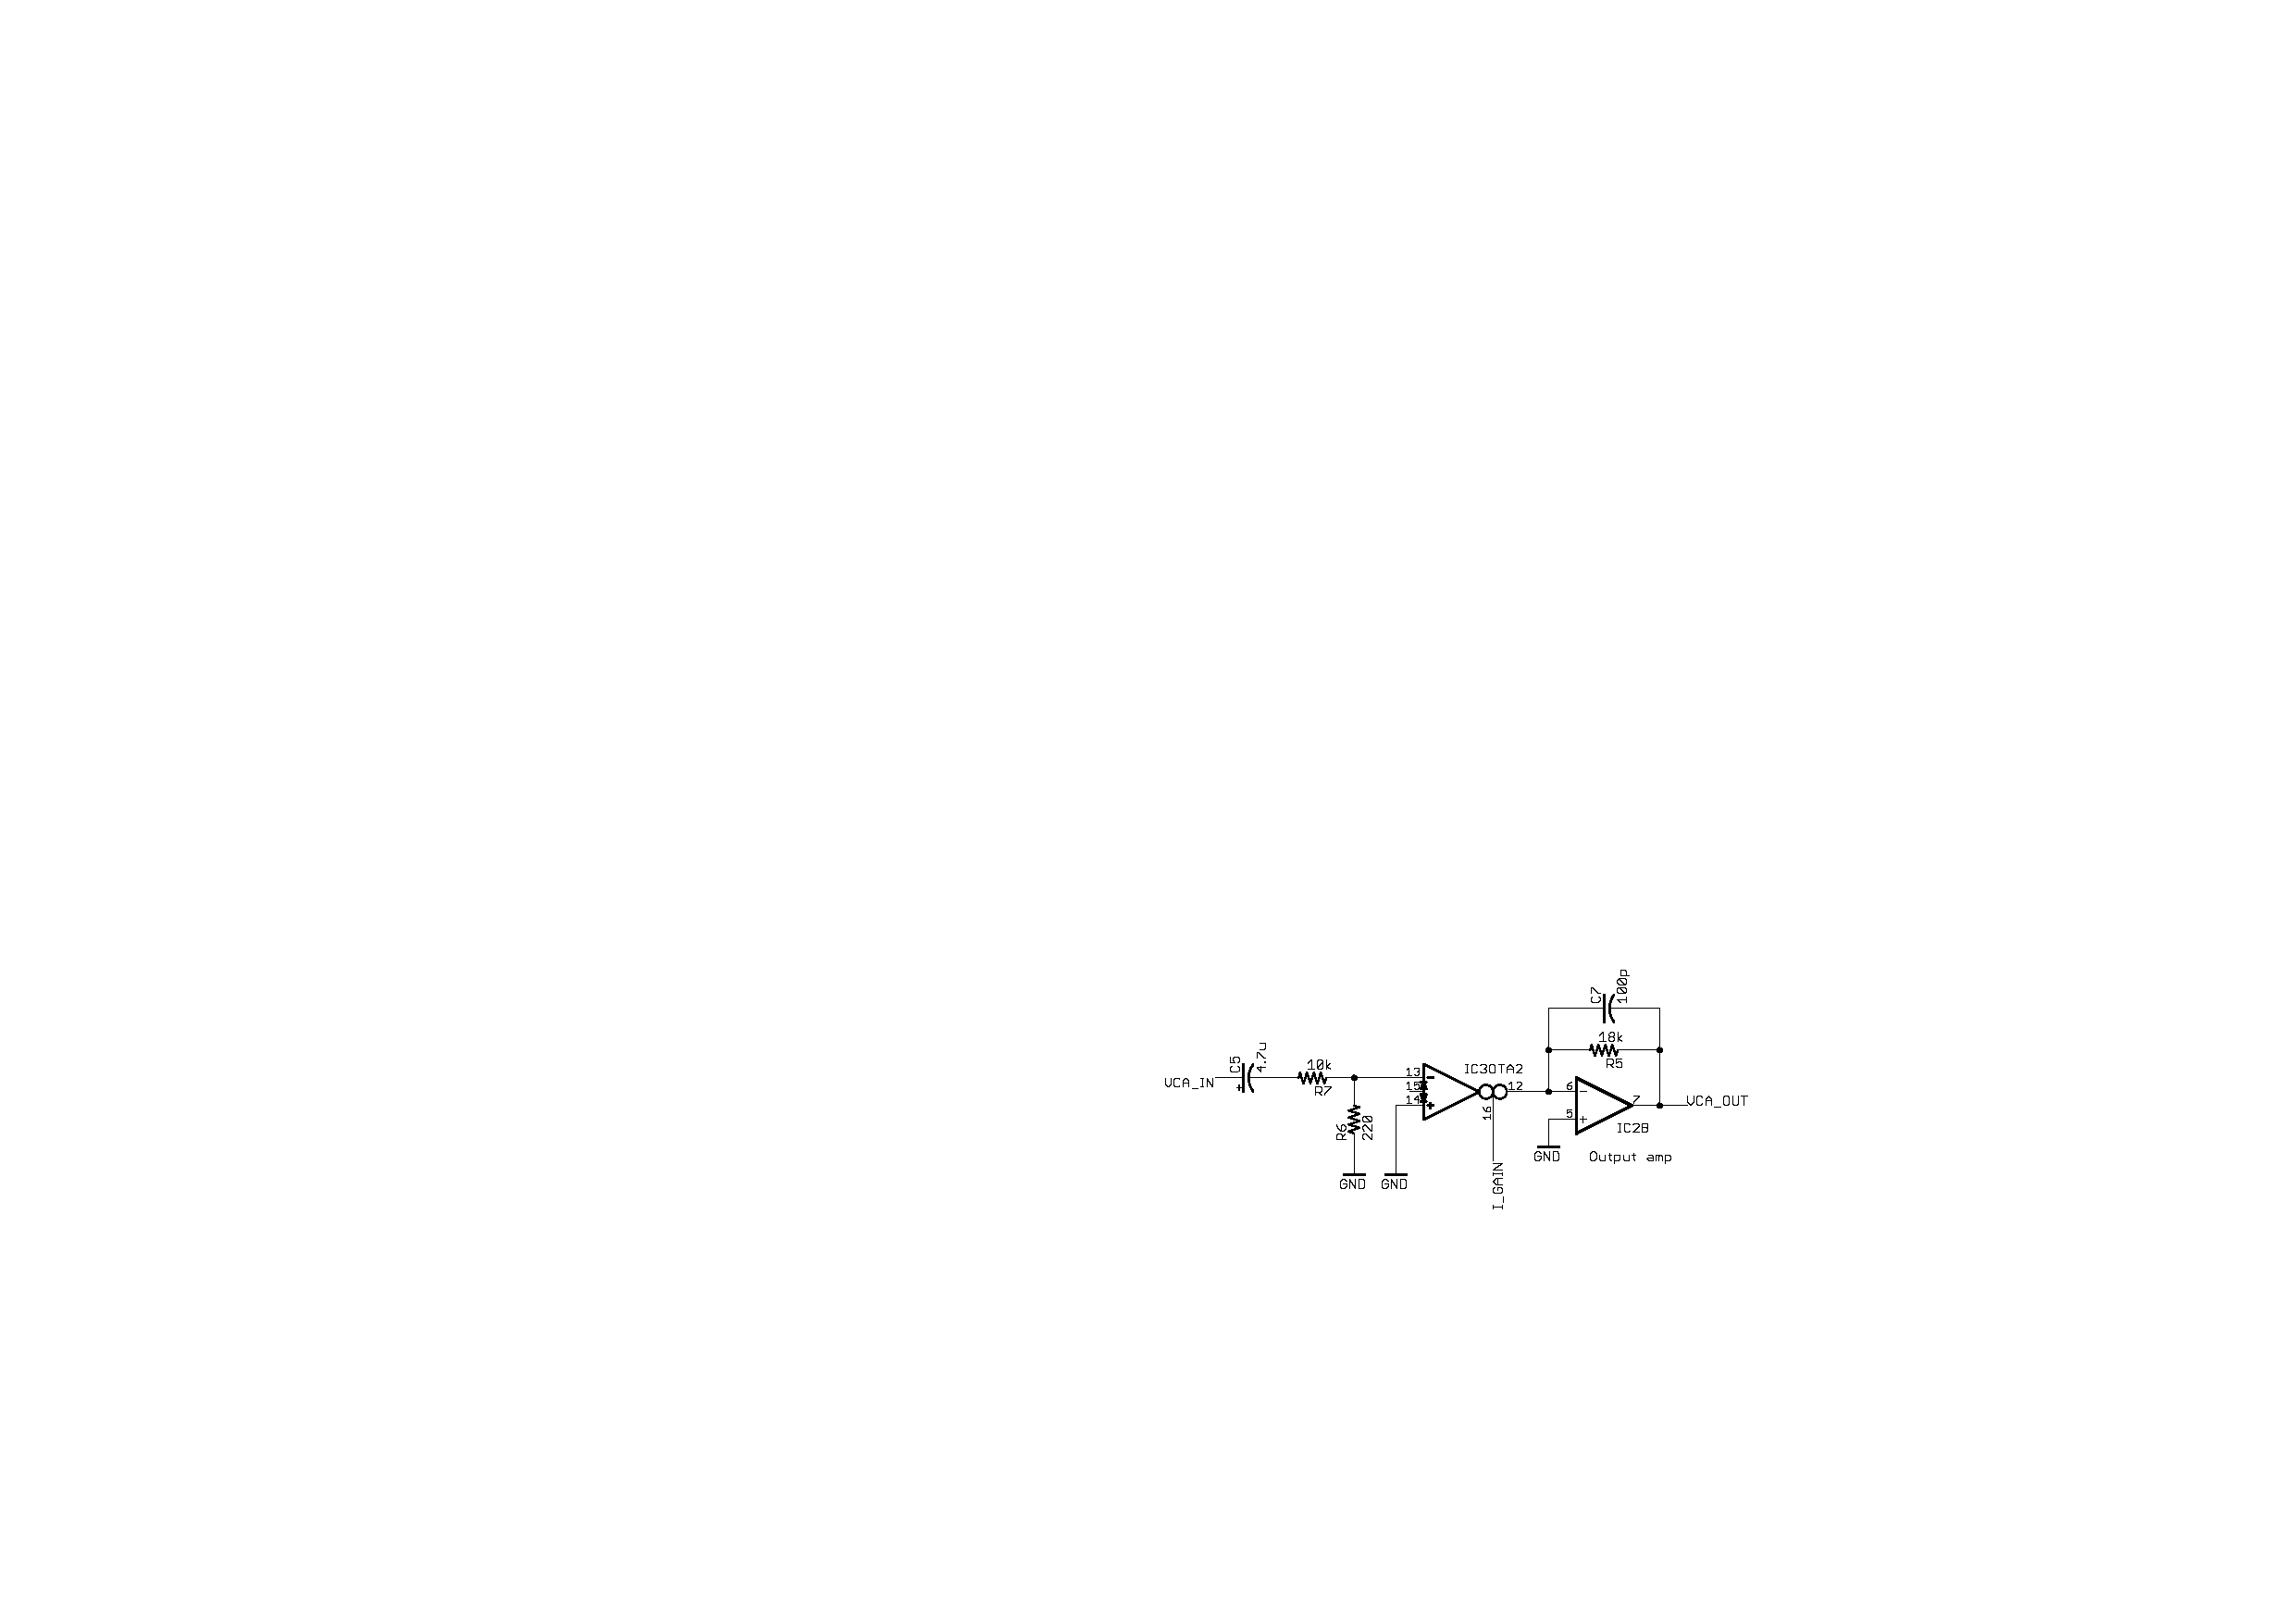
\includegraphics[width=0.8\textwidth]{smr4mkII_vca.pdf}
\caption{Current controlled amplifier.}
\label{fig:vca}
\end{figure}

The schematics in figure \ref{fig:vca} represents a current controlled amplifier.

$C5$ AC-couples the input. Assuming the input signal $VCA\_IN$ has no DC-offset, it can be ignored. The voltage at the inverting input of the OTA is:

\begin{equation}
V_- = \frac{R_6}{R_6 + R_7} VCA\_IN
\end{equation}

The current at the output of the OTA is:

\begin{eqnarray}
V_o &=& g_m (V_+(p) - V_-(p)) \\
 &=& -19.2 I_{gain} \frac{R_6}{R_6 + R_7} VCA\_IN
\end{eqnarray}

Finally, this current is converted into a voltage through $IC2B$ which works as a transimpedance amplifier:

\begin{equation}
VCA\_OUT = -R_5 V_o
\end{equation}

Using all these, the gain of the VCA is:

\begin{equation}
G = 19.2 R_5 \frac{R_6}{R_6 + R_7} \left(\frac{V_{gain}}{R_9} + \frac{V_{ee}}{R_{10}}\right)
\end{equation}

This yields a gain of $2$ when the $V_{gain}$ control signal is equal to its maximum value of $5V$.

\section{Resonance control}

Resonance is achieved by feeding back a fraction of the filter output signal into the filter input. Traditionally, this is done through a potentiometer (voltage divider). Here, in order to provide voltage control over resonance, we use a VCA similar in design to that of the main signal VCA. There are two important differences in the design:

First, the current output by the OTA is not converted back into a voltage by an op-amp. Instead, it is directly injected at the summing node of the first OTA-integrator cell. A way to look at it: the $220 \Omega$ resistor to ground at the OTA-integrator cell inverting input does the current to voltage conversion.

Then, the resonance VCA is fed not only with the filter output, but also with a fraction of the unfiltered input signal itself. This causes the level of the signal entering the filter to increase as resonance is increased, and helps in compensating the dreaded ``resonance loudness drop" of 4-pole filters. An extra refinement here is the the input signal is coupled into the resonance VCA through an undersized capacitor. This will cause the resonance loudness drop to be compensated only in the highest regions of the spectrum ; creating brighter and shinier sounds when the resonance is increased. This trick was inspired by the Jupiter-8 filter circuit.

\end{document}
